% For tips on writing the thesis, see http://www.tug.org/pracjourn/2008-1/mori/mori.pdf

% Two side to save paper
% openrigth means to put the chapter tittle on the right pages 
\documentclass[12pt,letterpaper,twoside,openright]{book}

% We define some strings that will use along
\def \thesiskeywords {Thesis, Operating Systems, Multimedia,  Embedded Systems, Linux, GStreamer, ARM, Davinci, OMAP}
\def \pdfauthor {Diego Dompe}
\def \thesistitle {Improving Operating Systems for Efficient Multimedia Handling in Embedded Systems}

% Custom-commands and definitions
% See this file for defining the keywords that will show up on the pdf file
% Language support
\usepackage[english,spanish]{babel}

%For spanish we need indentation on the first line
%\usepackage{indentfirst}

% Prevent latex from expanding to fill page
\raggedbottom

%Use the margins requested
\usepackage[hmargin={3.5cm,2.5cm},vmargin=2.5cm]{geometry}

%Improved bibliography
\usepackage{natbib}
\bibpunct{[}{]}{;}{n}{,}{,}

% To define spacing
\usepackage{setspace}

% We use these packages for making the nice logo on the title page
\usepackage[pdftex]{graphicx}

% Use input characters instead of scape codes
\usepackage[utf8x]{inputenc}

% Generate fancy chapter titles
\usepackage[Bjarne]{fncychap}

%Use Fancy headers
\usepackage{fancyhdr}

% Generate pretty PDF with links on the TOC
\usepackage{mdwlist}
\usepackage{alltt}
\usepackage[dvips, bookmarks=true,linktoc=all, colorlinks=false, pdftitle={\thesistitle}, pdfauthor={\pdfauthor}, pdfsubject={\thesistitle}, pdfkeywords={\thesiskeywords},
linkcolor=blue,filecolor=blue,urlcolor=blue,citecolor=blue]{hyperref}

% Allow epigraphs at the beginning of chapters
\usepackage{epigraph}

% Define abstract environment since it doesn't exists on book class
\newenvironment{abstract}%
{\cleardoublepage\null \vfill \begin{center}%
\bfseries \abstractname \end{center}}
{\vfill\null}

% Generation of nomenclature
\usepackage{nomencl}
\makenomenclature

% Generation of acronyms
\usepackage{acronym}

% For color definitions
\usepackage{color}

% Comment this out when is not a draft
%\usepackage{draftwatermark}
%\SetWatermarkLightness{0.95}
%\SetWatermarkFontSize{5cm}
%\SetWatermarkScale{5}
%\SetWatermarkText{DRAFT}

% Custom commands
\newcommand{\HRule}{\rule{\linewidth}{0.5mm}}


\begin{document}

% This is the first part of the document (frontmatter), use Roman numeration
\frontmatter

% Simple style
\pagestyle{empty}

\begin{titlepage}

\begin{center}


\includegraphics[width=0.3\textwidth]{../Common/Images/logoTec}
\\[0.2cm]
\definecolor{tecblue}{rgb}{0.016,0.173,0.322}
\textcolor{tecblue}{%
\textsc{\LARGE Escuela de Ingeniería en Computación}\\[0.2cm]
\textsc{\large Programa de Maestría en Computación}\\
 }
 \vfill
 
% Title
\HRule 
\\[0.9cm]
\doublespacing
{ \huge \bfseries \thesistitle}
\\[0.4cm]
\singlespacing
\HRule 
\\[1.4cm]

{\large Thesis Proposal\\
Submitted in partial fulfillment of the requirements for the degree of\\[0.6cm]
Magister Scientiæ en Computación}
\\
\vfill
 
 % Author and supervisor
\begin{minipage}{0.45\textwidth}
\begin{flushleft} \large
\textsc{Author:}\\
{Diego Dompe}
\end{flushleft}
\end{minipage}
\begin{minipage}{0.50\textwidth}
\begin{flushright} \large
\textsc{Advisor:}\\
{Francisco J. Torres-Rojas, Ph.D.}
\end{flushright}
\end{minipage}
 
 
\vfill
 
% Bottom of the page
{\large August 2011}
 \end{center}
 \end{titlepage}


% Now let put the abstract in two languages
\selectlanguage{spanish}%
\begin{abstract}
\end{abstract}

\selectlanguage{english}%
\begin{abstract}
\end{abstract}

\selectlanguage{english}%


\tableofcontents
%\listoffigures
%\listoftables
% Table of Symbols and Nomenclature
%\printnomenclature

\mainmatter
% Use double space
\doublespacing
% Now fancy style
\pagestyle{fancy}
% Left the right header clean
\rhead{}

\chapter{Introduction and background}
\epigraph{People in the embedded space don't do prototypes. They hack something until it works, then it's done.}{xav user on lwn.net}

\section{Introduction}


\section{Background}
Embedded Systems are one of the fastest growing markets in the computer industry, with more than 10 billion embedded processors shipped in 2008 \citep{Clarke:2009uq}.

Embedded Software development is a discipline that is younger that software development for other environments like \acp{PC} or Mainframes. There are some particular issues that transform embedded software development into a complex eco-system:
\begin{itemize*}
\item It usually requires some level of integration with the hardware that is non-common in other software development areas.
\item Many of the hardware integration that is done is very particular and unique, which usually makes the code hard to re-use if isn't designed properly (or if the technology is new and isn't clear how to implement the software solution in a generic way).
\item The market for embedded system is so fast-paced that developers are in pressure to deliver working devices as soon as possible. Few companies care about the quality or re-usability of their embedded code, except by hardware vendors or efforts from single open-source minded developers who want to contribute back. For example recent articles regarding status of the contributions to the Linux™ kernel for the ARM architecture the contributions status as a  ``mess'' due many of the different interests and agendas behind it \cite{Proffitt:2011fk}.
\item Many embedded developers may lack formal training on software development, but instead have an \ac{EE} background.
\end{itemize*}

These factors usually means that embedded developers will not likely find or apply the same best-practices that the rest of the software industry use. Is not rare to find embedded projects where each revision of the same product will have a complete new software stack or re-implementation from the previous iteration.

The fact that the code is tailored for specific hardware to the point where it can't be easily re-used goes against \acp{OS} theory which proposes that the \ac{OS} should abstract all the software from the hardware implementation \citep[p.~29]{Silberschatz:2010vn}. However many embedded devices (especially ones with low memory footprint) may use a custom-made \ac{OS} or use no \ac{OS} at all (also called an \ac{OS}-less solutions).

On embedded systems capable enough to support it, Linux has gradually gained acceptance as an \ac{OS} for embedded systems due his open-source nature and support from embedded processors manufacturers, especially on the \ac{SoC} market. \acp{SoC} are the main trend for new product development in recent years due the benefits it brings to new chip development \citep{Somaya:2000fk}.

The advantages that Linux provides for new embedded product development are clear:
\begin{itemize*}
\item It's a probed \ac{OS} which has been successfully used in different embedded markets.
\item No royalty fees or licenses cost associated directly with it (although some embedded vendors may add royalty fees if you use their custom distributions).
\item Wide knowledge base available and many developers are familiarized with it.
\item Usually hardware companies provide drivers and support for Linux in their latest devices (for example ethernet or wireless circuits, storage devices, etc.), simplifying the integration of hardware components for an embedded system. This is a critical element for minimizing the time-to-market of a product.
\end{itemize*}

However Linux also presents some disadvantages for the embedded space:
\begin{itemize*}
\item It's not designed to be a \ac{RTOS}, which make it not suitable for all type of embedded applications.
\item There is a learning curve for \ac{RTOS} developers, since Linux enforces some concepts that may be foreign to them:
	\begin{itemize*}
	\item Memory space protection: most \ac{RTOS} do not provide memory space protection.
	\item Separation between the kernel and user space applications: This is a side-effect of the memory space protection.
	\end{itemize*}
\item There are several algorithms used in non-\acp{RTOS} like Linux that may affect the performance compared to \acp{RTOS} or \ac{OS}-less solutions:
	\begin{itemize*}
	\item Context Switches: there is a penalty associated on several hardware architectures with the memory protection.
	\item I/O Scheduling: the kernel page cache may defer I/O work. Linux offers full control to customized this behaviors for embedded systems, but many developers may be unaware of them.
	\item Interrupts prioritization: mainline Linux kernel doesn't offer a way to control priorities for interrupt handlers. There are patches to transform interrupt handlers into kernel threads, but they aren't available for all kernel versions and may require specific analysis and tuning to achieve desired results \cite{Song_Chubb_10}.
	\end{itemize*}
\end{itemize*}

Despite the short-comings that Linux present versus a \ac{RTOS}, just the fact of have widely available drivers and software stacks for peripherals on the embedded space usually outweighs these problems. Many \acp{SoC} may require complex software stacks to interact with integrated peripherals, such is the case of heterogenous \acp{SoC} using a \ac{GPP} and a \ac{DSP} or other sort of hardware unit for accelerating specific operations (such as video coding, cryptographic algorithms, etc). Implementing or porting the functionality of these software stacks required to interact with the desired peripheral to an \ac{OS}-less or other non-supported \ac{RTOS} is usually non-effective in terms of cost or time.

However many developers that are un-familiar with Linux and/or general purpose \acp{OS} design, approach the task of implementing the functionality for their embedded products bypassing Linux functionality. For example the author of this work have found several times kernel drivers for Linux designed just to specifically allow user-space access to the peripherals by any user space application in commercial \ac{OEM}/\ac{ODM} offerings for embedded development (TODO publish code and put a reference).  There are several reasons for developers using this kind of approach:
\begin{itemize*}
\item Some times the software stack was designed in \ac{OS}-less environment and ported over to Linux. Developers just try to find a way to get the Linux hardware management out of the way of the software stack.
\item Developers are simple un-familiar with Linux design.
\item Linux may lack APIs or functionality to handle new scenarios posted by the hardware design. For example ability to realize zero-memory-copy operations.
\item Developers try to use Linux's APIs but found that performance was un-acceptable for unknown reasons. In the embedded community is widely believed that general proposes  \acp{OS} Linux may be unsuitable for certain embedded applications since is bloated for desktop systems.
\end{itemize*}

Another common believe in the embedded community is that any software design highly specialized will provide better performance than a implementing it over a generic solution. One example of this is multimedia software architectures on top of Linux, where the amount of data being processed requires to use data paths with zero memory copy operations across the whole software stack.
 
\section{Problem statement}
Many embedded developers tend to create software designs and architectures that aren't re-usable or maintainable for different reasons; one of them is the empiric premise that generic software architectures penalize performance. Furthermore there are little incentives from the product development cycle for embedded products to invest into optimizing the \acp{OS}. All these factors lead to creation of software platforms that are hard to reuse or leverage into future project versions or other projects, potentially increasing the costs of development.

This work focuses on the particular scenario of multimedia software systems for embedded systems and uses Linux on the ARM architecture.

\section{Hypothesis}
It it's possible to optimize general propose \aclp{OS} to provide good performance with negligible penalty compared to custom solutions where not \acl{OS} is used for multimedia software stacks in embedded systems.

\section{Previous work}
\subsection{Literature review}
Classic works:

exokernel: \cite{Engler95exokernel:an}

SPIN: \cite{Bershad95extensibility}

YIMA: \cite{Shahabi:2002vn}


It wasn't possible to find existing literature on the specific subject of this work, however we found related literature that may apply.

Liedtke \citep{Liedtke:1995kx} proved with his work that using the right algorithms and analysis it is possible to implement software stacks that manage hardware access with minimal performance penalties. He faced common belief that $\mu$-kernels suffer inherit design performance penalties and demonstrated that rather than a design issue it was an implementation issue the root cause of the performance problems. Liedtke also showed that architecture-specific optimizations were required without loosing generality in the software architecture design.

If we characterize the main differences between Linux and \acp{RTOS} or \ac{OS}-less solutions, we can identify previous work that addresses the performance and optimizations for these areas in embedded processors.

\cite{Plagemann2000267} Operating system support for multimedia systems

\cite{Regehr00operatingsystem} Operating System Support for Multimedia: The Programming Model Matters

\subsubsection{Memory Protection and Context Switching}

\citep{Chanteperdrix:2009fk}) implemented FASS

\citep{David:2007:CSO:1281700.1281703}  instrumented performance penalties associated with context-switching in ARM processor architecture.

\cite{Blackham_SH_11} Protected Hard Real Time

\subsubsection{I/O Handling}
\cite{Chu96zero-copytcp}: Zero copy tcp in solaris

Netwokring: \citep{Kim:2002:MCR:646603.697068}

Buffers and algorithms: \cite{Jane98enhancementsto}

Efective IO for RTP: \cite{springerlink:10.1007/s11390-006-0989-5}

\cite{Kim:2002:MCR:646603.697068} A Memory Copy Reduction Scheme for Networked Multimedia Service in Linux Kernel


\subsubsection{Process Scheduling}
TODO

\subsection{Software Stack}
Performance of Gstreamer: \cite{Contreras:vn} and obviously me: \cite{Dompe:2011ys}


\section{Long-Range Consequences}
This work will contribute to the analysis of the factors involved on measuring and improving performance the Linux kernel for his use on embedded systems dealing with multimedia software stacks.

\chapter{Objectives and Contributions}
\section{Objectives}
Focus on the benefits of your study not the research problem.
Place yourself in the position of responding to someone who says “so what?” Provide a persuasive rationale for your argument by answering the following questions: Why is your study important? To whom is it important? What can happen to society, or theory, or a program if the study is done or not done?

\subsection{Purpose}
Begin with “The purpose of this study is to…” change, interpret, understand, evaluate, or analyze the problem.
State your thesis goal completely. Remember, it should be some form of investigative activity.

\section{Previous work}

\subsection{Literature review}
Locate and briefly describe those studies and theories that support and oppose your approach to the problem. In other words, place the proposed study in context through a critical analysis of selected research reports.
Be sure to include alternative methodological approaches that have been used by others who studied your problem.

\subsection{Previous solutions}

\chapter{Methodology and Schedule} 
\epigraph{There is no greater harm than that of time wasted.}{Michelangelo}

\section{Methodology}
Tools for characterizing and analyzing performance on each specific scenario will be identified and integrated on the testing platforms. There are existing open source tools that provide the required information, but little information regarding specific use to instrument the desired scenarios.

The following are the specific scenarios that will be evaluated on each platform:
\begin{itemize*}
\item Video capture, and encoding.
\item Audio capture, and encoding.
\item Synchronized video and audio capture, encoding and storage in block-based storage devices using an standard multimedia file container.
\item Synchronized video and audio capture, encoding and transmission over network using RTP/UDP/IP protocol.
\item Video decoding and preview from block-based storage devices using a standard multimedia file container.
\end{itemize*}

For block-based storage devices, we consider any storage device with semantics similar to that of standard hard disks, and specifically excluding devices based on flash memory unless they use any sort of \ac{FTL}.

The following aspects will be considered for each specific scenario:
\begin{itemize*}
\item CPU usage and scheduling overhead.
\item Memory usage and overhead by the software stack.
\item I/O usage: efficiency regarding use of the specific I/O architecture and overhead by the software stack.
\end{itemize*}

\section{List of Deliveries}
The deliveries are:
\begin{enumerate*}
\item Patches for the Linux kernel available for the specific platforms to improve their performance.
\item Patches for GStreamer to improve performance on the target scenarios and platforms.
\end{enumerate*}

As stated previously, all the patches will be designed with the intention of being accepted into their respective projects, but no guarantee is made about their merging on mainstream. Still, the work will be done while interacting with the respective project maintainers.

\newpage
\section{Schedule and Work Breakdown}

\begin{table}[tph]
\caption{Work Breakdown} \centering
\begin{tabular}{c}
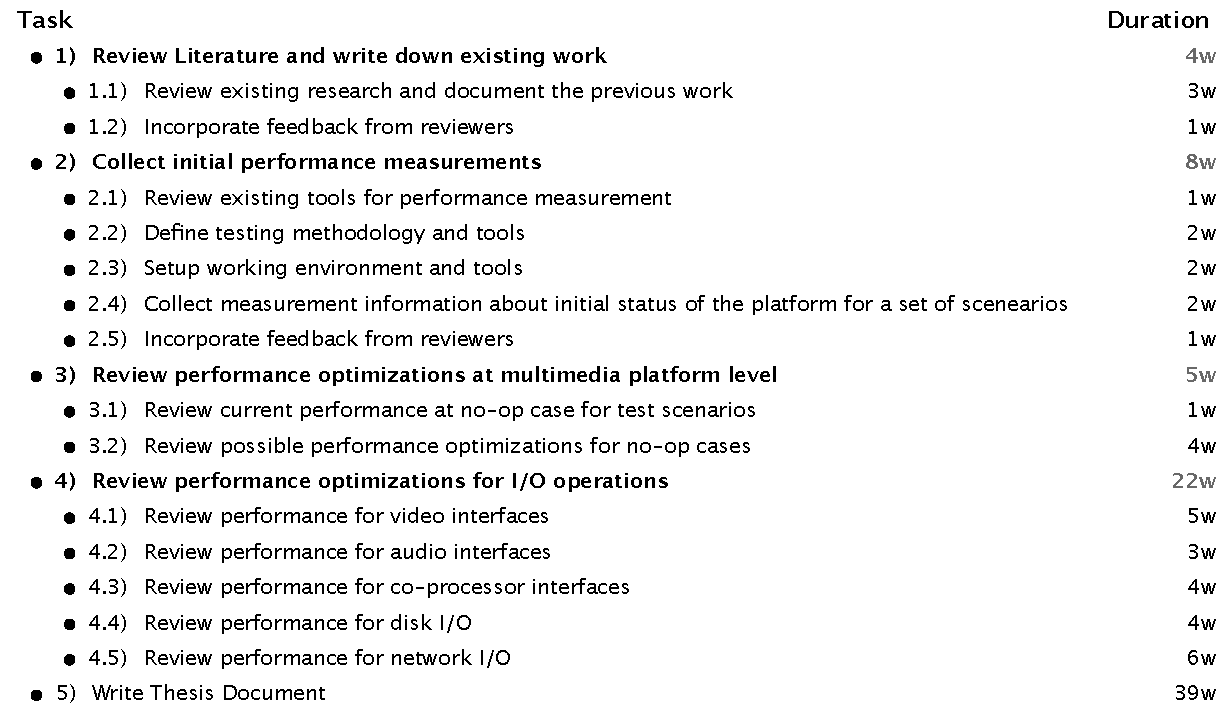
\includegraphics[width=1.0\textwidth]{images/Outline.pdf}
\end{tabular}
\end{table}

\begin{figure}[tbh]
\centering
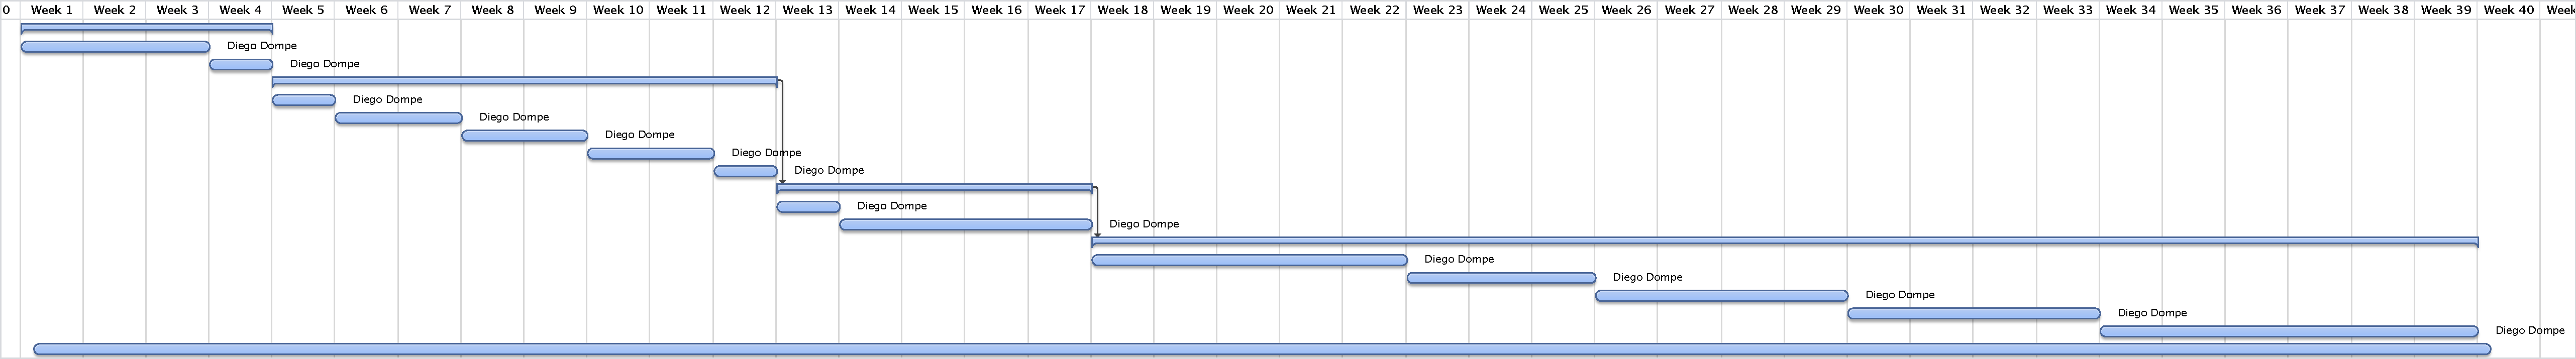
\includegraphics[width=0.55\textheight,height=0.34\textwidth,angle=90]{images/Gantt.pdf}\\
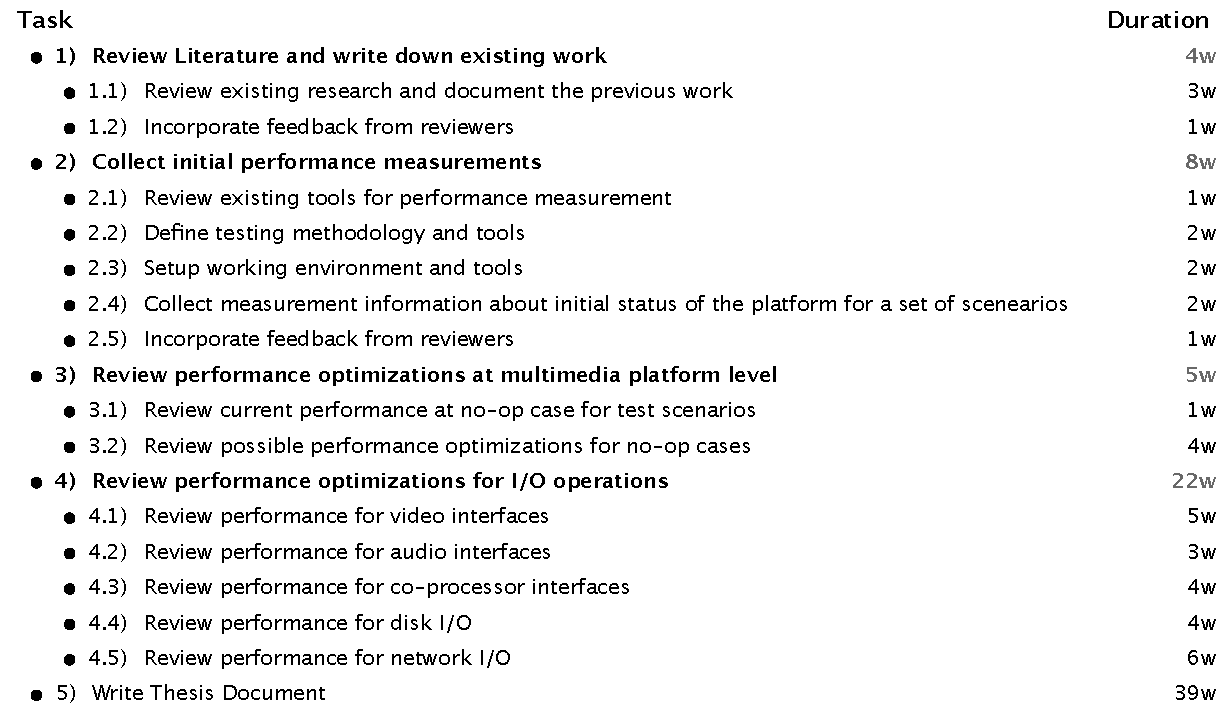
\includegraphics[width=0.4\textheight,angle=90]{images/Outline.pdf}
\caption{Gantt Chart}\label{gantt}
\end{figure}


% Appendixes
%\appendix 
%\input{Body/appendix1}

% Final pages
\backmatter

% Use single space
\singlespacing

% Bibliography
\cleardoublepage
\bibliographystyle{plainnat}
\refstepcounter{chapter}
\addcontentsline{toc}{chapter}{\bibname}
\bibliography{../Common/references.bib}

% Acronyms
\chapter{Acronyms}

% Please keep it sorted by alphabetical order
\begin{acronym}

\acro{DSP}{Digital Signal Processor} is a special type of micro processor.

\acro{EE}{Electronic Engineer}

\acro{GPP}{General Purpose Processor} is a processor suited for standard computational operations, in contrast of a \ac{DSP} for example.

\acro{OEM}{OEM (TODO)} 

\acro{OS}{Operating System}

\acro{PC}{Personal Computer}

\acro{RTOS}{Real Time Operating System} is an operating system that is designed to meet with Real Time deadlines.

\acro{SoC}{System on a Chip} is a technology that consist on integrating several functional blocks of re-usable electronics logic (even from different vendors) into single die.


\end{acronym}



\end{document}
